\documentclass{article}

\usepackage{graphicx}
\usepackage[left=2cm, right=2cm, top=2cm]{geometry}

\begin{document}

% The following part of this document will be placed in the Methods section

This final simulation for the binary lens demonstrates a range of plots,
which are all successful in modeling the number of images and magnification
for the smallest possible mass ratios within the scope of my project. More
specifically, the plots show the same grids for varying mass ratio, $q$, and
separation, $s$, in the planet frame, using the Skowron and Gould 2012 root
solver.

As of this point in the project, I have determined that doing calculations
in the planet frame and using the Skowron and Gould 2012 root solver produces
the least error-prone calculations. This final simulation for the binary
lens demonstrates the most extreme values of the mass ratio, $q$, with
typical values of separation, $s$, for which we can accurately model the
number of images and the magnification. This simulation was therefore
calculated in the planet frame, using the root solver in Skowron and Gould
2012. \textbf{Figure 1} shows the plot of the number of images, and
\textbf{Figure 2} shows the plot of the magnification.

\begin{figure}
	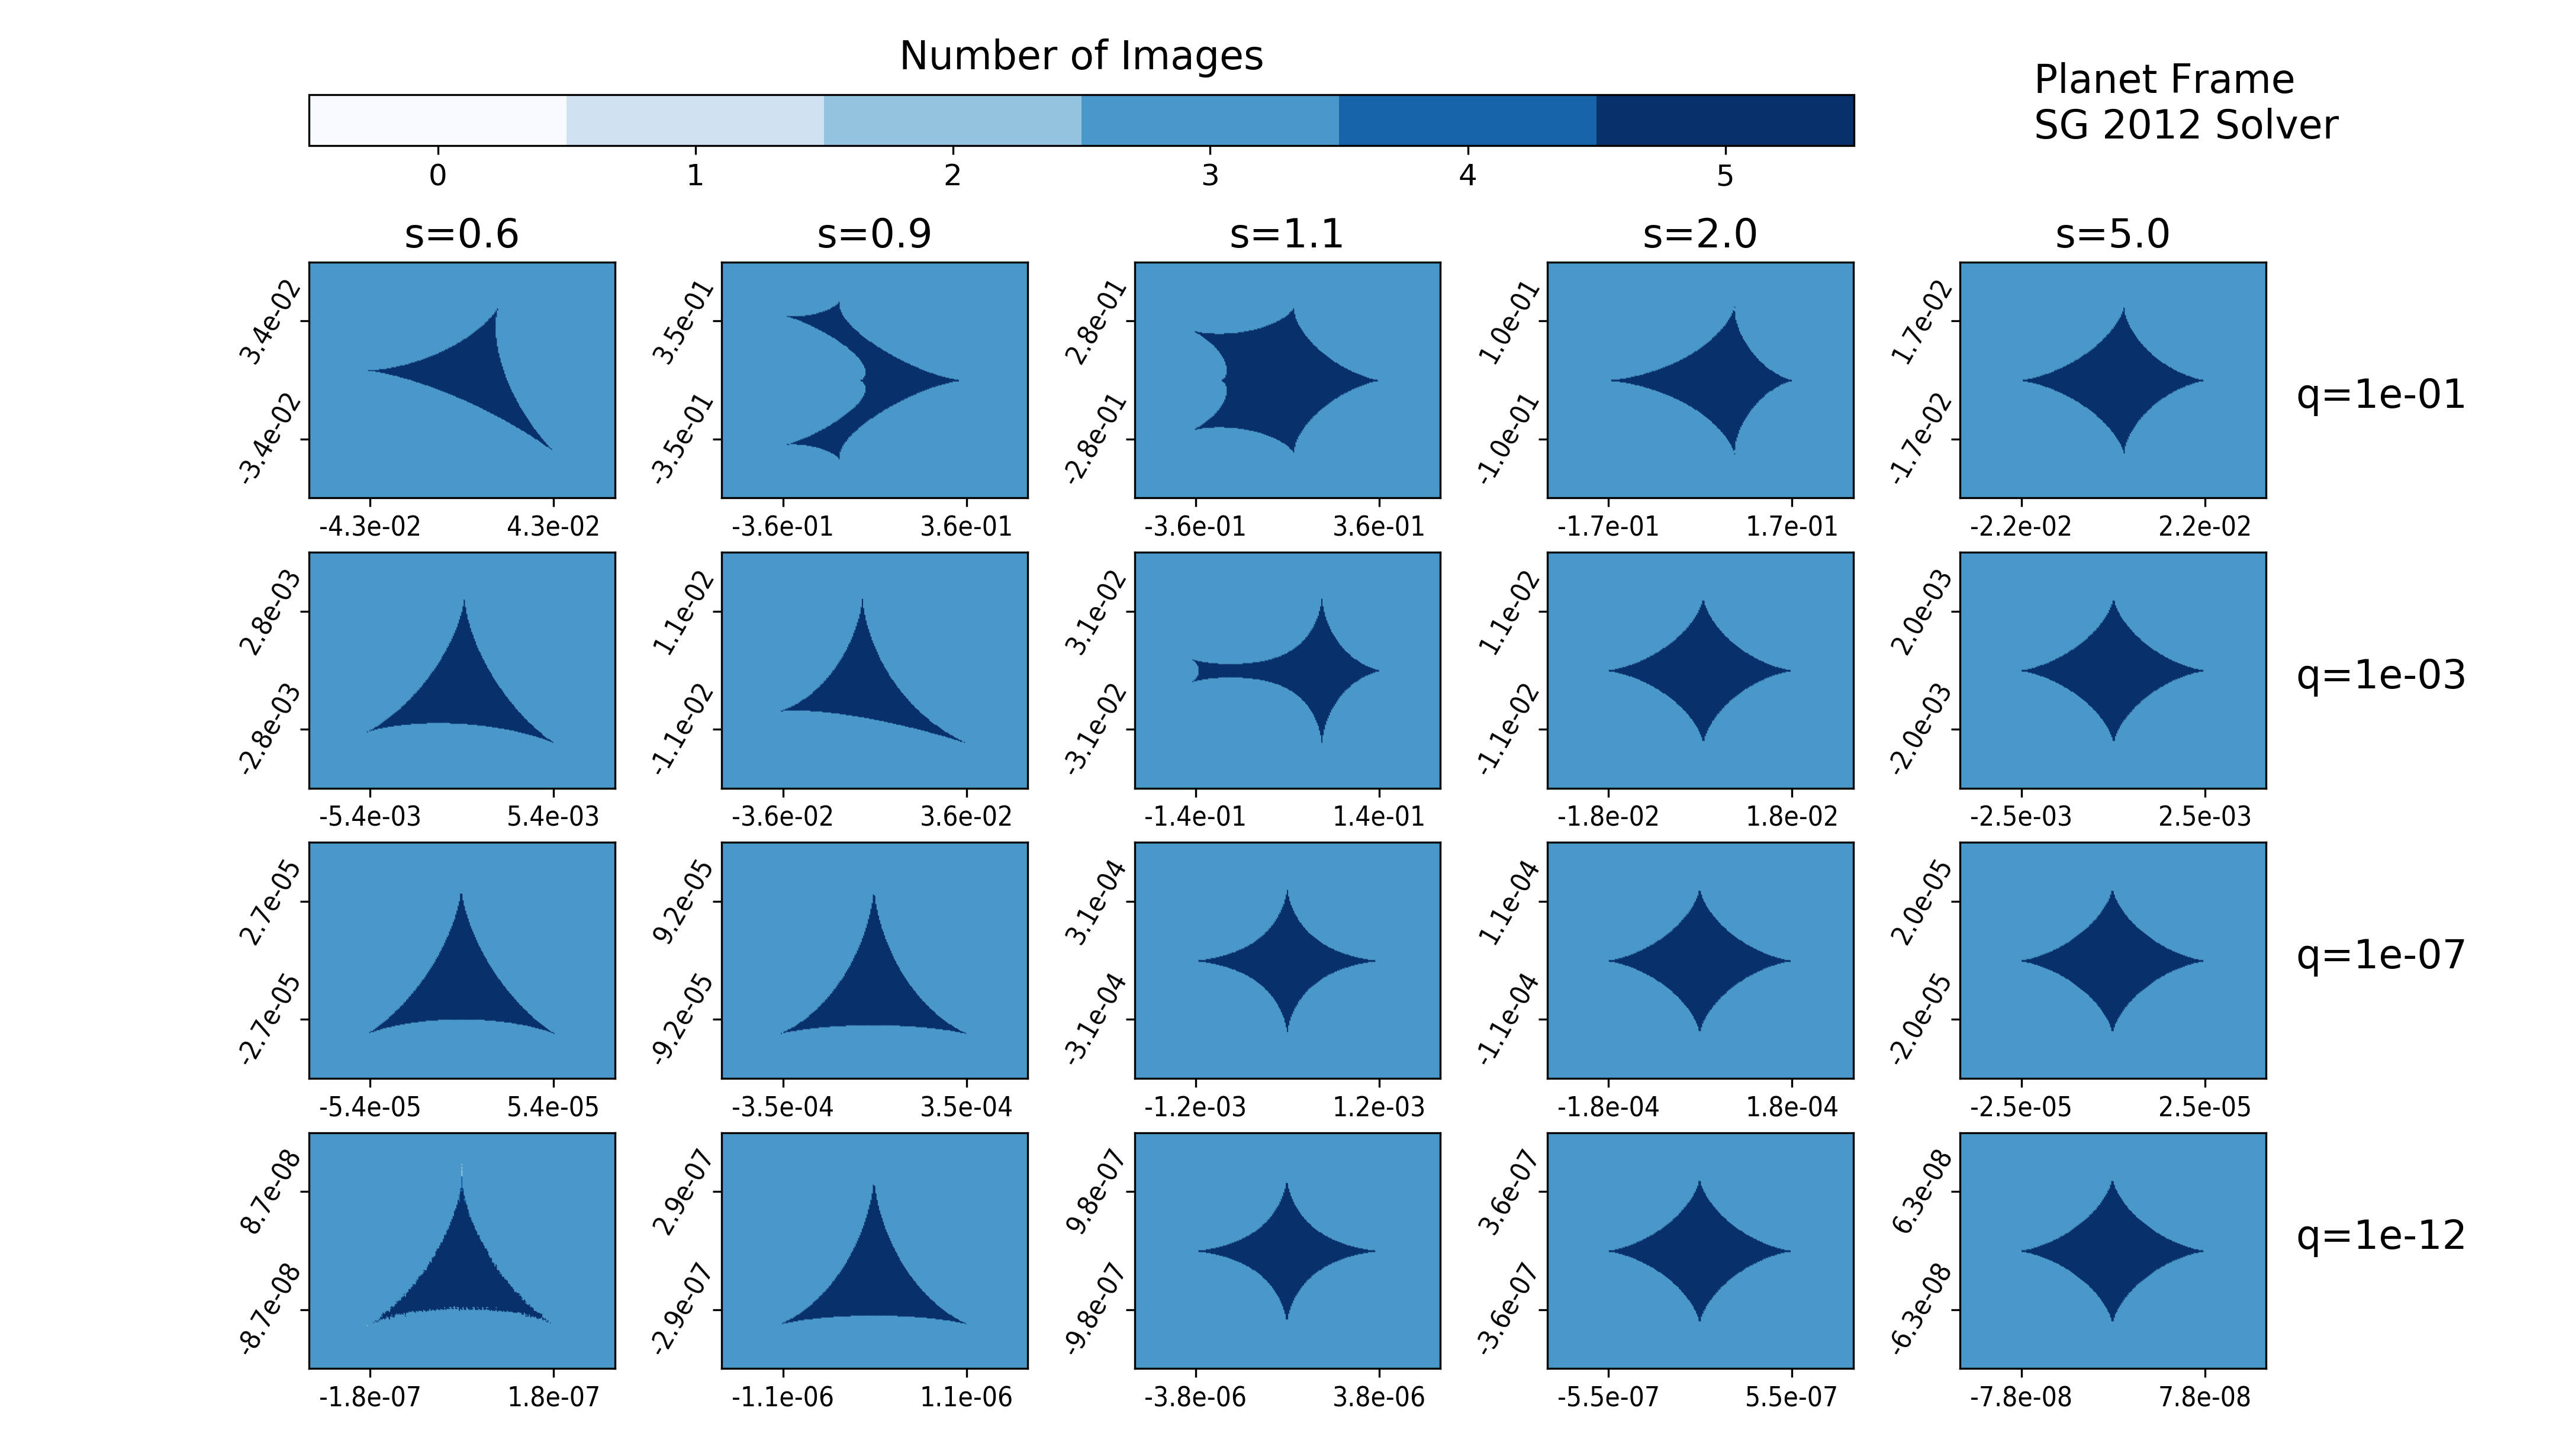
\includegraphics[width=0.9\textwidth]{../Tables/images_plan_0.png}
	\caption{The number of images versus the position for varying parameters
	$q$ and $s$. All plots are accurate, with no errors, thus demonstrating
	the lower limit of what a typical computer can successfully calculate
	for binary lensing events.}
\end{figure}

\begin{figure}
	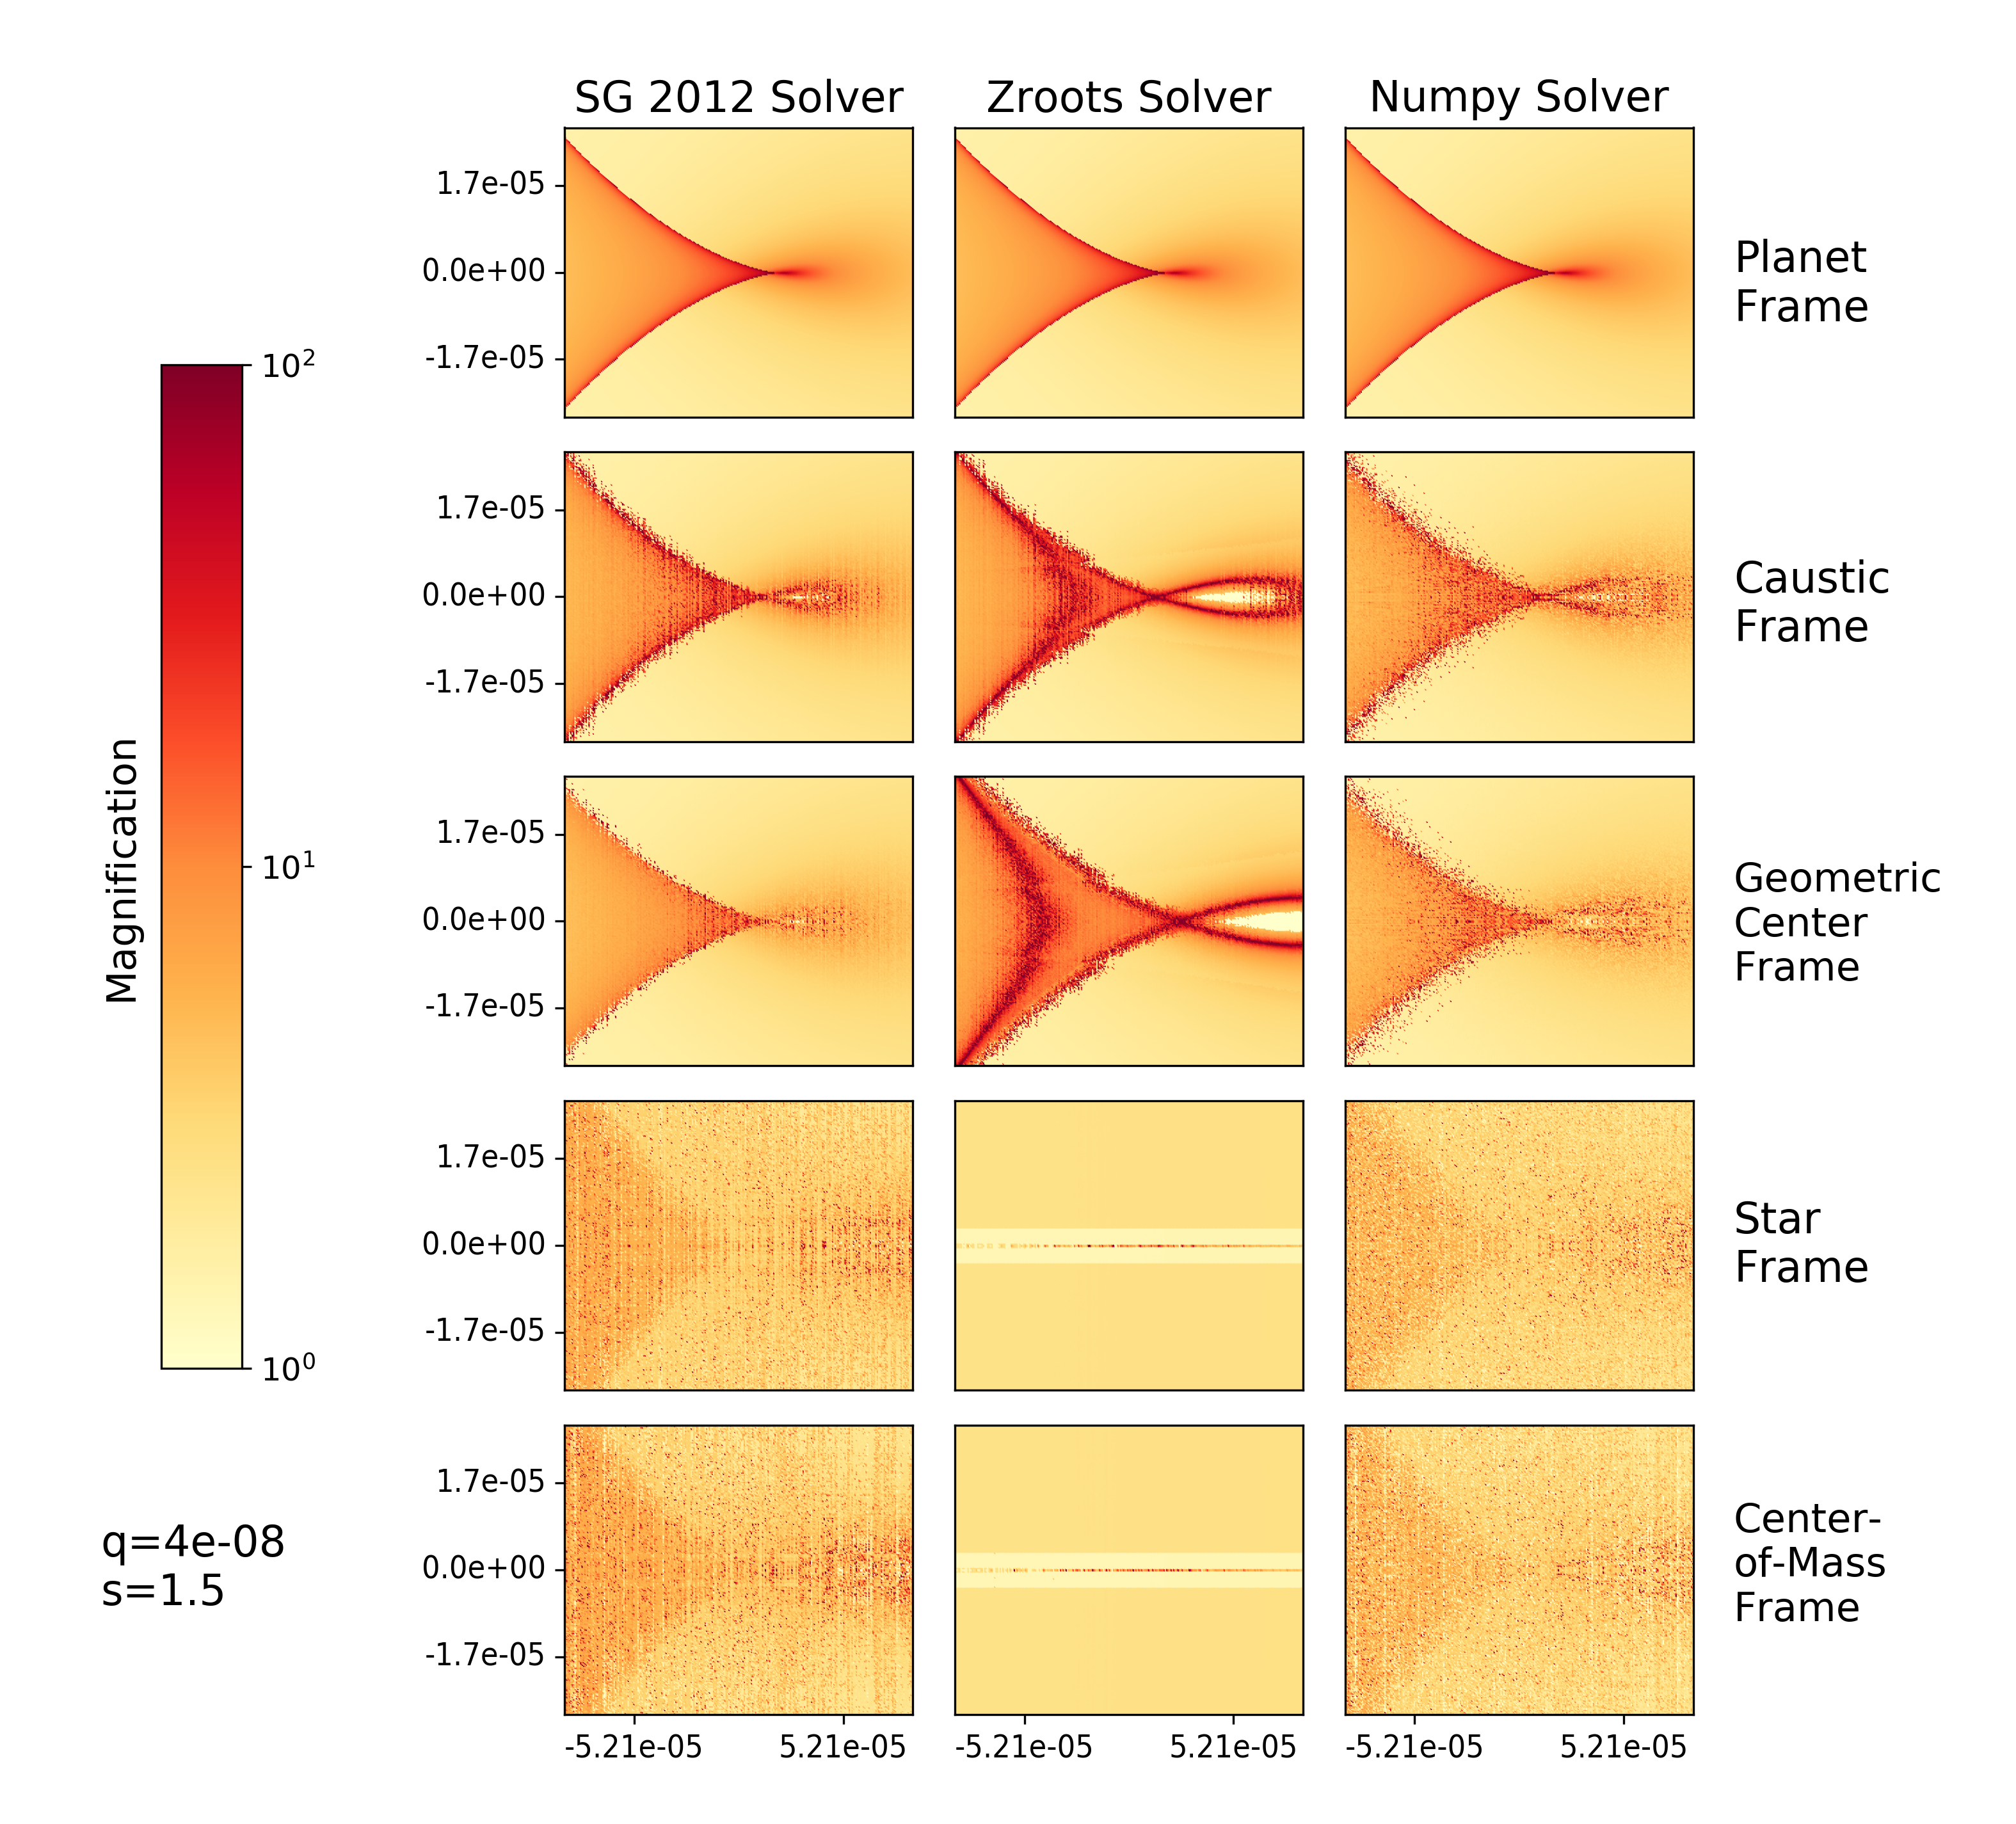
\includegraphics[width=0.9\textwidth]{../Tables/magn_solver_0.png}
	\caption{Same as \textbf{Figure 1}, except with magnification.}
\end{figure}

% The following part of this document will be placed in the Results/Analysis
% section

This simulation suggests that we can successfully model binary lensing
events for mass ratios all the way down to $q=10^{-12}$ for a wide range of
separations between the host star and planet. This number drops to
$10^{-15}$ for values of $s$ between $~1.2$ and $5$. This is far more
precise than modern technology will be able to detect, which suggests
researchers do not need to rely on more precise and time-consuming
algorithms than those mentioned in this project.

\end{document}
